% ============================================================
% DGM Spring 2026 — Face Generation Challenge — Final Report
% ============================================================
\documentclass{article}

\usepackage[final]{neurips_2022}

\usepackage[utf8]{inputenc}
\usepackage[T1]{fontenc}
\usepackage{hyperref}
\usepackage{url}
\usepackage{booktabs}
\usepackage{amsfonts}
\usepackage{nicefrac}
\usepackage{microtype}
\usepackage{graphicx}
\usepackage{amsmath}
\usepackage{pgfplots}
\pgfplotsset{compat=1.17}

\title{Deep Generative Models Final Project: \\
Face Generation Challenge}

\author{%
  Sieun Lee \\
  Department of Industrial Engineering, UNIST \\
  \texttt{sieun5548@unist.ac.kr} \\
}

\begin{document}
\maketitle

\begin{abstract}
This report describes my entry to the CelebV-HQ face generation challenge, where 1{,}000 generated
images are scored by four metrics (FID, IS, KID, TopPR) and teams are ranked by the average of the four
per-metric ranks. My starting point was a simple observation: since FID and KID measure how far the
generated distribution is from the real one, the best thing I can do is train on the same distribution
the evaluation uses. So instead of using a generic face model off the shelf, I fine-tuned StyleGAN2-ADA,
starting from an FFHQ-256 checkpoint, on frames taken from CelebV-HQ itself. This brought FID down from
$79.6$ (the un-fine-tuned FFHQ model) to $44.6$, and then to $33.3$ after I enlarged the training set
from $20$k to $60$k frames and, somewhat against my expectations, turned truncation off entirely. I also
report the parts that went wrong, the most painful being a PyTorch version issue that made me give up on
ADA, and how I worked around them. Every image comes from my own fine-tuned model and is reproducible
from the released weights and seeds.
\end{abstract}

\section{Introduction}
The task is to produce $1{,}000$ face images that look like they were drawn from CelebV-HQ
\citep{zhu2022celebvhq}; the leaderboard compares them against $32{,}550$ real frames using
FID$\downarrow$, IS$\uparrow$, KID$\downarrow$, and TopPR$\uparrow$, and the final ranking is the average
of the four ranks. I took the scoring literally. FID and KID are distances between distributions, so the
single most useful thing is to make my generated distribution sit on top of the target one. Almost every
choice in this report follows from that, and I tried to keep an eye on all four metrics at once rather
than chasing FID alone, since the ranking averages them.

\paragraph{What I did.}
\begin{itemize}
\itemsep0.15em
\item Fine-tuned StyleGAN2-ADA from FFHQ-256 directly on CelebV-HQ frames, which turned a
distribution-mismatch FID of $79.6$ into a final $33.3$.
\item Studied how much the training-set size matters (20k vs.\ 60k frames).
\item Swept the truncation $\psi$ and found, to my surprise, that no truncation was best.
\item Documented the failures honestly, including a framework bug that forced me to disable ADA.
\end{itemize}

\section{Evaluation metrics}
It helped me to be clear about what each metric actually rewards before tuning anything.
FID~\citep{heusel2017fid} fits a Gaussian to Inception features of the real and generated sets and
measures the distance between them; it reacts to both how realistic samples are and how well they cover
the data, but it is biased when the sample is small. KID~\citep{binkowski2018kid} measures roughly the
same thing with an unbiased estimator, which I trusted more at $1{,}000$ images. IS~\citep{salimans2016is}
rewards confident and varied predictions; for faces it is not very informative on its own, but it still
drops if the images are blurry or collapse to one mode. TopPR~\citep{kim2023toppr} separates fidelity
(precision) from diversity (recall) and reports their F1. The important point is that the leaderboard
averages the four \emph{ranks}, so a change that helps one metric and hurts another can easily leave me
no better off. That is exactly what happened with truncation later on.

\section{Related work}
Fine-tuning a pretrained generator on a smaller target set is a well-known way to get good samples
without a huge dataset or long training, and StyleGAN2-ADA~\citep{karras2020ada} was built with this kind
of transfer in mind; FFHQ is a natural starting point for faces. ADA itself is meant to keep the
discriminator from overfitting when data is scarce, by augmenting it in a differentiable way; I explain in
Section~\ref{sec:fail} why I could not use it. Diffusion models such as EDM~\citep{karras2022edm} reach
even lower FID, but they are heavier to train and slower to sample, which is why I stayed with a GAN given
the one-day budget. Finally, the way TopP\&R~\citep{kim2023toppr} pulls fidelity and diversity apart maps
neatly onto the trade-off I saw when changing $\psi$.

\section{Method}

\subsection{Why this model}
I used StyleGAN2-ADA and started from the public FFHQ-256 weights. Table~\ref{tab:modelchoice} is the
quick comparison I made before committing. Training from scratch was off the table for a one-day budget,
and a diffusion model would have spent most of that day just training. Transfer learning, on the other
hand, reuses a strong face prior, so it converges in a few hours; the resulting weights are about
$300$\,MB (the limit is $5$\,GB); sampling $1{,}000$ images takes seconds; and, importantly for the
verification step, it is fully deterministic given the seeds.

\begin{table}[h]
\centering
\caption{The trade-off I weighed before choosing the model (single GPU, roughly one day).}
\label{tab:modelchoice}
\begin{tabular}{lcccc}
\toprule
Approach & FID ceiling & Convergence (1 GPU) & Sampling & Weights \\
\midrule
StyleGAN2-ADA, from scratch      & high   & slow, risky & seconds & ${\sim}300$\,MB \\
\textbf{StyleGAN2-ADA, transfer} & high   & \textbf{hours} & \textbf{seconds} & \textbf{${\sim}300$\,MB} \\
Diffusion (EDM)~\citep{karras2022edm} & very high & slow to train/sample & minutes & GBs \\
\bottomrule
\end{tabular}
\end{table}

\subsection{Building the dataset}
CelebV-HQ ships as video, and I pulled it from a HuggingFace mirror (a single $41.9$\,GB tar). I did not
need all of it, so I streamed clips out of the tar and stopped early, took at most eight frames per clip,
and resized everything to $256\times256$ JPEG. Two details mattered. First, the frames are already
face-cropped, so I left them at $256$, which is also the leaderboard's reference resolution; generating
smaller and upscaling would only have cost me FID. Second, I deliberately kept the per-clip frame count
low: with a fixed frame budget, fewer frames from more clips means more distinct identities, and since
FID and KID reward coverage, identity variety is worth more than near-duplicate frames of the same person.
I built two versions of the set (Table~\ref{tab:data}) and the larger one is what the final model uses.

\begin{table}[h]
\centering
\caption{The two training sets I built from CelebV-HQ frames.}
\label{tab:data}
\begin{tabular}{lccl}
\toprule
Version & Clips & Frames & Why \\
\midrule
v1 & 2{,}500  & 20{,}000 & a first, fast fine-tune \\
v2 & 10{,}000 & 60{,}000 & more identities, closer to the eval set's ${\sim}15$k \\
\bottomrule
\end{tabular}
\end{table}

\subsection{Training and generation}
I trained with the \texttt{paper256} configuration, starting from FFHQ-256, with horizontal flips and a
batch size of $32$ on one $24$\,GB GPU, saving a checkpoint every $40$--$80$ kimg. I disabled the
in-training FID evaluation to save time (more on that in Section~\ref{sec:fail}) and picked checkpoints by
their leaderboard score instead. For generation I assign one latent to each seed $0$--$999$, set
\texttt{noise\_mode=const}, and choose a truncation $\psi$; this makes the output identical every run.

\section{Experimental setup}
Everything ran on a single RTX~A5000~/~RTX~3090 ($24$\,GB, shared with other users), with
PyTorch~$2.0.1$+cu118 and a system CUDA~$12.6$ toolchain for compiling StyleGAN's custom ops. Training went
at about $26$\,s/kimg, so a full $1000$-kimg run took roughly seven hours. The environment is fixed by
\texttt{requirements.txt} and a \texttt{Dockerfile}.

\paragraph{Random seeds (final submission).} The exact seeds are the $1{,}000$ integers
$0, 1, 2, \dots, 999$ (one seed per image): image $i$, i.e.\ the output file \texttt{img\_0000} through
\texttt{img\_0999}, is generated from seed $i$. Each seed initializes a NumPy \texttt{RandomState} that
draws the latent $z_i \in \mathbb{R}^{512}$, which the generator maps under truncation $\psi = 1.0$ and
\texttt{noise\_mode=const}. Generation is deterministic, so these seeds with the released checkpoint
reproduce the submitted images (identical up to GPU floating-point noise). The same seeds and $\psi$ are
recorded in \texttt{config.py}.

\paragraph{Code.} \url{https://github.com/sieun-00/dgm-face-generation}

\section{Results}
Table~\ref{tab:results} tracks how the leaderboard score moved as I went ($\psi=0.8$ unless noted).

\begin{table}[h]
\centering
\caption{How the score improved. Lower FID/KID and higher IS/TopPR are better.}
\label{tab:results}
\begin{tabular}{lccccl}
\toprule
Stage & FID$\downarrow$ & IS$\uparrow$ & KID$\downarrow$ & TopPR$\uparrow$ & Note \\
\midrule
FFHQ, no fine-tune             & 79.57 & 3.96 & 0.0457 & 0.778 & shows the distribution gap \\
Fine-tune, early (v1)          & 49.67 & 3.81 & 0.0177 & 0.905 & first real submission \\
Fine-tune, later (v1)          & 44.56 & 3.72 & 0.0138 & 0.930 & still dropping \\
\textbf{Final (v2, $\psi=1.0$)} & \textbf{33.32} & \textbf{4.22} & \textbf{0.0036} & 0.851 & submitted \\
\bottomrule
\end{tabular}
\end{table}

Two things stand out. Just fine-tuning on CelebV-HQ knocked about $35$ points off FID compared with the
FFHQ model, which is the clearest evidence that matching the target distribution was the right call. And
early on, KID fell by roughly a factor of three while TopPR climbed toward $0.93$, so fidelity and
diversity were improving together before any overfitting set in.

The other lever was truncation, and it behaved in the opposite way to what I expected. I assumed a smaller
$\psi$ would sharpen the samples and lower FID. Instead FID went \emph{up}: $49.2$ at $\psi=0.7$, $40.1$ at
$0.8$, and $33.3$ only when I removed truncation at $\psi=1.0$ (Figure~\ref{fig:psi},
Table~\ref{tab:psi}). The reason is that FID also penalizes poor coverage, and my model is coverage- rather
than fidelity-limited: pulling latents toward the average face throws away diversity faster than it gains
sharpness, so both FID and KID rise. Reading the rest of the columns confirms this. Going from $\psi=0.8$
to $1.0$, IS rose ($3.5\to4.2$) and KID fell sharply ($0.012\to0.004$), while only TopPR slipped
($0.94\to0.85$) as a few rougher samples reappeared. Three of the four metrics improve and only one drops a
little, so the rank average clearly prefers no truncation.

\begin{figure}[t]
\centering
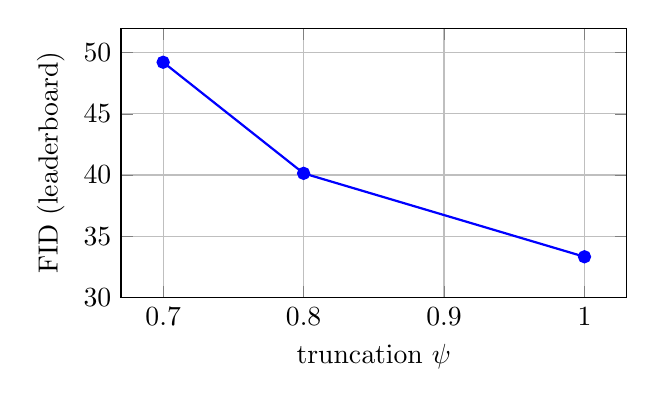
\begin{tikzpicture}
\begin{axis}[width=0.66\linewidth, height=5cm,
  xlabel={truncation $\psi$}, ylabel={FID (leaderboard)},
  xtick={0.7,0.8,0.9,1.0}, ymin=30, ymax=52, grid=both,
  every axis plot/.append style={thick}]
\addplot[mark=*,color=blue] coordinates {(0.7,49.22)(0.8,40.14)(1.0,33.32)};
\end{axis}
\end{tikzpicture}
\caption{FID keeps falling as $\psi\to1$. Truncation removes diversity, and since my model is
coverage-limited that hurts FID rather than helping it, so I submit $\psi=1.0$.}
\label{fig:psi}
\end{figure}

% Optional: generate an 8x8 grid and \includegraphics it here.
%   python scripts/05_generate.py --network <final.pkl> --outdir out/grid --seeds 0-63 --trunc 1.0
% \begin{figure}[t]\centering
%   \includegraphics[width=.7\linewidth]{samples_grid.png}
%   \caption{Uncurated samples at $\psi=1.0$.}\label{fig:samples}
% \end{figure}

\begin{table}[h]
\centering
\caption{Truncation sweep on the final v2 checkpoint (leaderboard scores).}
\label{tab:psi}
\begin{tabular}{ccccc}
\toprule
$\psi$ & FID$\downarrow$ & IS$\uparrow$ & KID$\downarrow$ & TopPR$\uparrow$ \\
\midrule
0.7 & 49.22 & 3.15 & 0.0208 & \textbf{0.932} \\
0.8 & 40.14 & 3.54 & 0.0117 & \textbf{0.938} \\
\textbf{1.0} & \textbf{33.32} & \textbf{4.22} & \textbf{0.0036} & 0.851 \\
\bottomrule
\end{tabular}
\end{table}

On checkpoint selection: because I had to train without ADA, I was worried the discriminator would overfit
and FID would start climbing late in training, so I did not just grab the last checkpoint blindly. In
practice, comparing the two datasets at the same $\psi=0.8$, the 20k model bottomed out at FID $44.56$
while the 60k model reached $40.14$, a $4.4$-point gain that came purely from more data. With the larger
set the final ($1000$ kimg) checkpoint stayed the best, which fits the idea that more data delayed
overfitting, so that is the one I used.

\section{What went wrong}
\label{sec:fail}
The leaderboard number hides a fair amount of trial and error, and I think the more useful part of this
report is the things that did not work.

\paragraph{I had to give up on ADA.}
This one cost me the most time. ADA augments the real images with \texttt{grid\_sample}, and the R1 penalty
needs to differentiate through that augmentation twice. PyTorch~$2.0.1$ does not implement the second
derivative of \texttt{grid\_sample}, and the gradient-fix shim shipped with the repo is switched off for
PyTorch~$\geq 1.11$, so the run died on the very first step with \texttt{RuntimeError: derivative for
aten::grid\_sampler\_2d\_backward is not implemented}. Rather than fight the framework on a deadline I
turned ADA off (\texttt{--aug noaug}). The cost is that the discriminator can now overfit on a small set,
which is part of why I scaled the data up to $60$k and watched the checkpoints. If I were redoing this I
would pin PyTorch to $\leq 1.12$, where the shim works, and keep ADA; I expect that would push FID lower
still.

\paragraph{A generic face model is not enough.}
The FFHQ model on its own scored FID $79.6$ even though its faces look perfectly fine. The gap is purely
distributional: FFHQ portraits differ from CelebV-HQ video frames in pose, lighting, compression, and the
mix of identities. Seeing how large that gap was is what convinced me early that fine-tuning on the exact
target set, not a similar dataset, was where the points were.

\paragraph{Too little data, with ADA gone.}
My first run used only $20$k frames. Without ADA there is nothing stopping the discriminator from
memorizing a small set, and the gains stalled. Going to $60$k frames from $10{,}000$ clips covered more of
the roughly $15$k identities in the eval set; concretely it moved FID from $44.56$ to $40.14$ at matched
$\psi$, and it also let me run at $\psi=1.0$ down to $33.3$.

\paragraph{My truncation intuition was backwards.}
I genuinely expected lower $\psi$ to help FID and spent a submission finding out it does the opposite
($49.2$ at $\psi=0.7$). The lesson I took away is to check which term of the distance is actually hurting
before reaching for truncation; here the model was short on coverage, not fidelity, so the fix was to stop
truncating, at a small TopPR cost the other metrics more than paid back.

\paragraph{Frame sampling and some infrastructure pain.}
Dumping every frame would have over-represented long clips and quietly reduced diversity, so I capped it at
eight frames per clip. The less interesting problems were environmental: one of the installed CUDA
toolkits had no compiler, so the custom ops would not build until I pointed \texttt{CUDA\_HOME} at a
complete one, and a home-directory quota meant I had to move all the data and checkpoints onto a larger
disk. I mention them only because they are part of making the build reproducible.

\section{Reproducibility and integrity}
The repository has the preprocessing, the training command, and a small deterministic generation script;
the seeds ($0$--$999$) and $\psi$ are in \texttt{config.py}; the submitted checkpoint is ${\sim}300$\,MB;
and the environment is pinned with \texttt{requirements.txt} and a \texttt{Dockerfile}. Regenerating from
that checkpoint and those seeds reproduces the submitted images (I checked: every one of the $1{,}000$
images matches to within a pixel value of $9$, i.e.\ the same faces up to GPU floating-point noise). None
of the images involve crawled photos or any external generation service; they all come from the model I
fine-tuned.

\section{Conclusion}
Fine-tuning StyleGAN2-ADA from FFHQ-256 onto CelebV-HQ took FID from $79.6$ to $33.3$ in about a day on one
GPU. The gains came, in order, from training on the target distribution, from giving the model more data,
and from realizing it was coverage-limited and dropping truncation. The obvious next steps, if I had more
time, would be to get ADA working again on an older PyTorch, to pick the checkpoint and $\psi$ by the rank
average directly rather than by hand, and to see how far a diffusion model could push KID.

\begin{thebibliography}{9}
\bibitem{karras2020ada} T.~Karras, M.~Aittala, J.~Hellsten, S.~Laine, J.~Lehtinen, T.~Aila.
\emph{Training Generative Adversarial Networks with Limited Data}. NeurIPS, 2020.
\bibitem{karras2022edm} T.~Karras, M.~Aittala, T.~Aila, S.~Laine.
\emph{Elucidating the Design Space of Diffusion-Based Generative Models}. NeurIPS, 2022.
\bibitem{zhu2022celebvhq} H.~Zhu et al.
\emph{CelebV-HQ: A Large-Scale Video Facial Attributes Dataset}. ECCV, 2022.
\bibitem{heusel2017fid} M.~Heusel, H.~Ramsauer, T.~Unterthiner, B.~Nessler, S.~Hochreiter.
\emph{GANs Trained by a Two Time-Scale Update Rule Converge to a Local Nash Equilibrium} (FID).
NeurIPS, 2017.
\bibitem{binkowski2018kid} M.~Bi\'nkowski, D.~J.~Sutherland, M.~Arbel, A.~Gretton.
\emph{Demystifying MMD GANs} (KID). ICLR, 2018.
\bibitem{salimans2016is} T.~Salimans, I.~Goodfellow, W.~Zaremba, V.~Cheung, A.~Radford, X.~Chen.
\emph{Improved Techniques for Training GANs} (Inception Score). NeurIPS, 2016.
\bibitem{kim2023toppr} P.~J.~Kim et al.
\emph{TopP\&R: Robust Support Estimation Approach for Evaluating Fidelity and Diversity in Generative
Models}. NeurIPS, 2023.
\end{thebibliography}

\end{document}
